\chapter{Related Work}
The following chapter presents state-of-the-art approaches and projects related to user mobility modeling and traffic analysis. These projects are used to derive the mobility of mobile subscribers by investigating events in mobile operator networks. They differ from classical behavior analysis in terms of penetration and accuracy. To derive the behavior of the entire population surveys and origin-destination matrices have been used in traffic modeling since the early 1960s~\cite{Beckmann,Heanue1966,Voorhees}.

Starting in the late 1990s floating phone data (FPD) has gained interest in traffic estimation and congestion detection. FPD are used due to its high penetration rate e.g.\, the market penetration in Austria was $159\%$\footnote{Press conference by the Forum Mobilkommunication \href{http://www.fmk.at/Medien/Pressekonferenzen/FMK-Jahrespressekonferenz-2012}{press conference link}} in 2013. There is a large volume of published studies describing the role of FPD for traffic analysis \cite{Yim2001,Qiu2007,Caceres2008}.

The approaches that will be presented here have a higher penetration rate due to the fact that they investigate a whole network whereas surveys can only cover parts of the entire network. Since surveys consists of a limited sample, they only cover a part of the whole population. Another advantage of these approaches is the adaption to seasonal changes. Surveys only depict the behavior at a certain point in time. However both road and mobile network traffic modeling depend on changes in time. By exploring events in mobile operator networks, the behavior can be analyzed for every point in time.

\subsubsection{Evaluation of a cellular phone-based system for measurements of traffic speeds and travel times: A case study from Israel}
To measure the traffic speed and travel time in Israel Bar-Gera~\cite{Bar2007} used a proprietary system by Estimotion Ltd. The system works with handover updates to derive the traveled route and traffic speeds. A sequence of locations derived from the handover footprint is matched to road segments which appear to be the most likely on the road network. An example of a handover sequence and its footprints on the road network is shown in Figure~\ref{fig:bar}. Despite the fact that this is a proprietary system it gives a good overview of the capabilities of floating phone data. The work by Bar-Gera shows that travel time estimation with phone data can be a replacement for loop magnetic detectors. He investigated a road segment from January to March 2005 and found that the average absolute difference between the two systems is $10.7\%$. However the whole system has its limitations due to the noise generated by floating phone data. They could reduce the noise by combining travel speeds from subscribers that traveled on the same road segment.
\begin{figure}
\centering
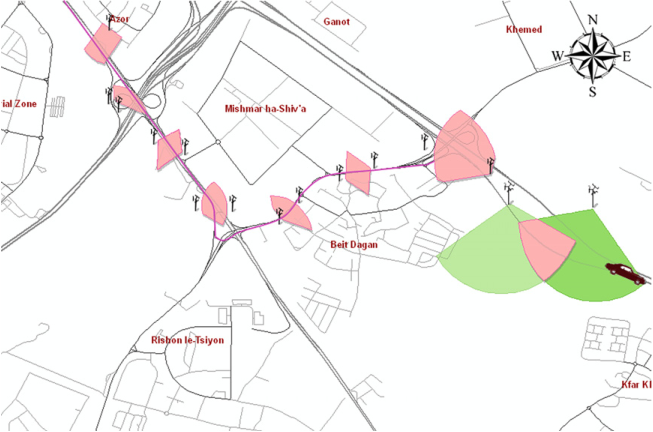
\includegraphics[width=\linewidth]{images/bar}
\caption{Handover sequences and footprints generated by a moving vehicle~\cite{Bar2007}}
\label{fig:bar}
\end{figure}

\subsubsection{Generating Trajectories from Mobile Phone Data}
To derive trajectories form mobile subscribers Schlaich~et al. \cite{Schlaich2010a} used location area sequences. Location area update events are issued whenever a mobile subscriber enters a new location area. These events are issued in both connected and idle states. Therefore trajectories can be generated even when no call is ongoing. Due to the small number of location areas in the research area, each location area was represented by a unique character. The next step was to generate routes in the research area and store the location area characters for each area they traversed. To estimate a trajectory for a mobile subscriber the location area sequence for the subscriber was compared to route sequences that have been generated before. Figure~\ref{fig:schlaichcomp} depicts the comparison of a mobile subscriber sequence and route sequences with high similarity.
\begin{figure}
\centering
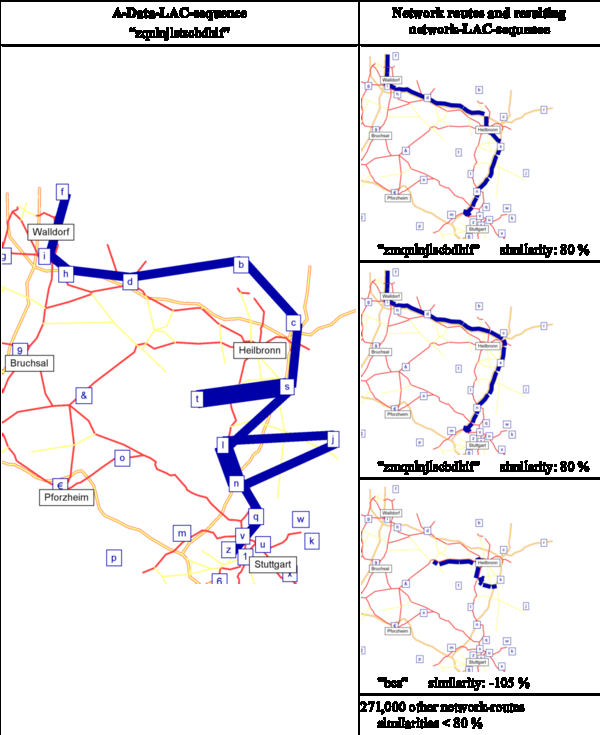
\includegraphics[width=0.7\linewidth]{./images/schlaichcomp}
\caption{Results of comparison between sequences with high similarity by Schlaich~et al.~\cite{Schlaich2010a}}
\label{fig:schlaichcomp}
\end{figure}
The results showed that this technique works well for longer trips around 20 kilometers because trips can only be estimated if the number of different location areas is greater than 3. Schlaich~et al.\ also stated that the presented approach only generates trajectories for SIM cards and not for vehicles. A vehicle can have none, one or more SIM cards therefore a vehicle can generate $0..n$ trajectories where $n$ is the number of SIM cards within the vehicle.


\subsubsection{Route Choice Estimation Based on Cellular Signaling Data}
To overcome the use of origin-destination matrices Tettamanti~et al.\ \cite{Tettamanti2012} used a simulation framework and a route generator to generate trajectories for mobile subscribers. Instead of using location area updates as Schlaich~et al.\ did they used handover updates. Handover updates allow to generate trajectories not only for a higher road network but also for the minor one. Their approach is based on cell area estimation as each handover update reveals the current cell area. Whenever a mobile phone reaches the boundary of the currently connected cell or when another cell has a higher reception then a handover is made to a cell with a better reception. Tettamanti~et al.\ used Voronoi partitioning to calculate the coverage area for each cell site to estimate a coarse user position.

The main limitation when using handover updates is that a handover update is only propagated when the mobile phone is in connected mode (during a call).

The start and end of the trajectory were set by the centroid of the cell where the call originated and terminated. To derive routes, a traffic modeling simulation framework VISSIM was used. VISSIM was used to generate routes between the start and the end of the call. For each of the generated routes, the euclidean distance between each of the cell sites and the generated route was calculated. To compare different routes equation~\ref{eq:sumsquare} was used  as a metric. For each route $j$, the squared sum of all minimum distances $d_{i,j}$ between the route and the cell site was calculated. The route with the minimum sum was used as a trajectory for the subscriber.
In Figure~\ref{fig:tettaroutes} an example for four different routes which were generated by VISSIM can be seen. Table~\ref{tab:tetta} depicts the results of the above stated equations (see Equation~\ref{eq:sumsquare}). In this example route 4 (see Figure~\ref{fig:tettaroutes}(d)) had the smallest squared sum of all four routes.

\begin{equation}
\label{eq:sumsquare}
D_j=\sum_{i=1}^{m} d_{i,j}^{2}
\end{equation}
\begin{equation}
\label{eq:minsum}
min(D_j), j = 1,2,\ldots,n
\end{equation}



\begin{figure}
	\centering
	\begin{subfigure}[b]{0.5\linewidth}
		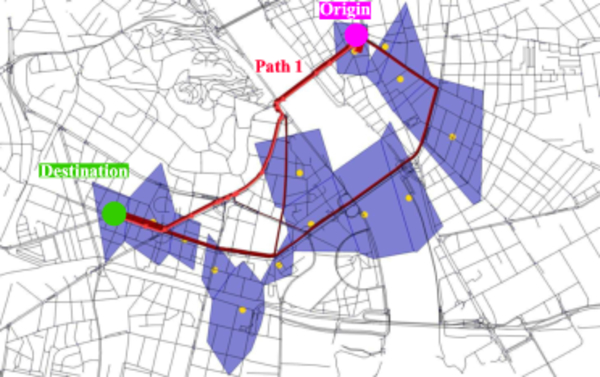
\includegraphics[width=\textwidth]{./images/tattipath0}
		\caption{}
		\label{fig:tattipath0}
	\end{subfigure}%
	~
	 %add desired spacing between images, e. g. ~, \quad, \qquad etc.
	%(or a blank line to force the subfigure onto a new line)
	\begin{subfigure}[b]{0.5\linewidth}
		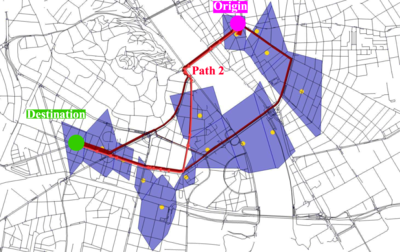
\includegraphics[width=\textwidth]{./images/tattipath1}
		\caption{}
		\label{fig:tattipath1}
	\end{subfigure}

	\begin{subfigure}[b]{0.5\linewidth}
			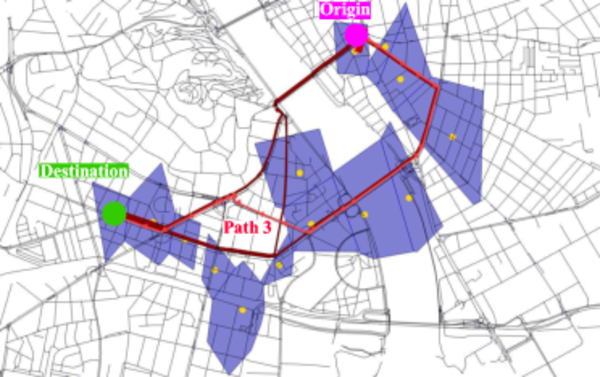
\includegraphics[width=\textwidth]{./images/tattipath2}
			\caption{}
			\label{fig:tattipath2}
		\end{subfigure}%
		~
		 %add desired spacing between images, e. g. ~, \quad, \qquad etc.
		%(or a blank line to force the subfigure onto a new line)
		\begin{subfigure}[b]{0.5\linewidth}
			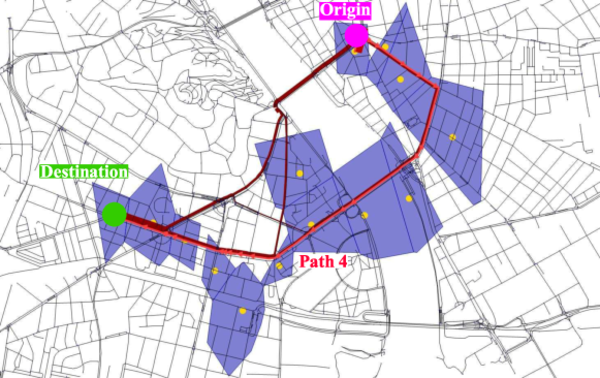
\includegraphics[width=\textwidth]{./images/tattipath3}
			\caption{}
			\label{fig:tattipath3}
		\end{subfigure}

	\caption{Comparison of four different generated routes, the best route was (d) by Tettamanti~et al.\ \cite{Tettamanti2012}}\label{fig:tettaroutes}
\end{figure}


\begin{table}[ht]
%\begin{tabular}{l|lp{3cm}|lp{3cm}}
%\hline
%Route $j$                   & $\sum _{i=1}^{m}{d}_{i,j}$ & Ratio compared to
%the lowest value & $D_j=\sum_{i=1}^{m} d_{i,j}^{2}$ & Ratio compared to
%the lowest value  \\ \hline
%1&6695&3.4&5130283&8.2 \\
%2&4519&2.3&3097741&4.9 \\
%3&2962&1.5&1356076&2.2 \\
%\textbf{4}&\textbf{1958}& 1  &\textbf{627122} &1 \\ \hline
%\end{tabular}

\begin{tabular}{l|ll}
\hline
Route $j$                   &  $D_j=\sum_{i=1}^{m} d_{i,j}^{2}$ & Ratio compared to
the lowest value  \\ \hline
a&5130283&8.2 \\
b&3097741&4.9 \\
c&1356076&2.2 \\
\textbf{d}  &\textbf{627122} &\textbf{1} \\ \hline
\end{tabular}
\caption{Squared deviations for each route as observed by Tettamanti~et al.\ \cite{Tettamanti2012}}
\label{tab:tetta}
\end{table}

The research by Tettamanti~et al.\ showed that trajectories can be generated for mobile subscribers by analyzing their handover events. This can be done without using special equipment and can be used to investigate the travel behavior of many subscribers.

\subsubsection{RoadCell -- Road Traffic Estimation from Cellular Network Signaling}
By using cellular network monitoring and therefore mobile subscription data Valerio et al.~\cite{Valerio2009,Valerio20092} at the FTW Forschungszentrum Telekommunikation Wien GmbH are investigating road networks in Austria. \emph{RoadCell}\footnote{Project website: \url{http://www.ftw.at/forschung-innovation/projekte/roadcell} last accessed March 12 2014} is using the same mobile subscription data source as our system~\cite{RoadCell2009}. The aim of \emph{RoadCell} is to recognize situations in the traffic flow by analyzing events in the core network of the mobile network operator. Driven by the fact that each road user is also a subscriber of a cellular network, network operator can be seen as another source to gather traffic information. Their motivation is to provide road operators with an inexpensive toolkit to observe the traffic flow without the installment of costly sensors. Thereby it is possible to not only investigate the traffic flow on the higher road network but also on minor roads where the installment of dedicated sensors is not cost-effective.

The idea is to observe changes in network signaling events and extract road conditions for example: drop in the handover rate; abrupt change in the LR update; increase in the number of calls/SMS; change in the number of road users. Figure~\ref{fig:raodcell_accident} shows how an accident effects the amount of Routing Area Update (RAU) and Location Area Update (LAU). An accident is indicated by a sharp decrease in RAU and LAU events followed by a sharp increase in RAU an LAU events.
\begin{figure}
\centering
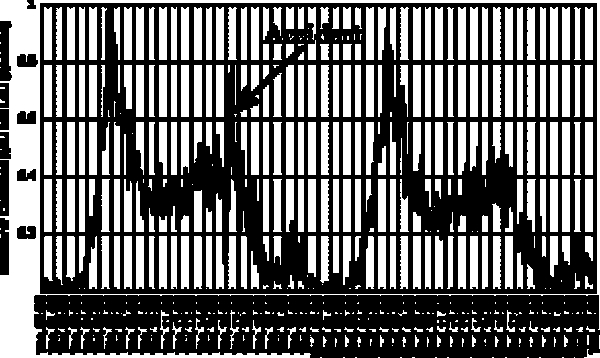
\includegraphics[width=0.7\linewidth]{./images/raodcell_accident}
\caption{Effect of the accident on the number of combined RAU and LAU; tic=300s \cite{Valerio20092}}
\label{fig:raodcell_accident}
\end{figure}

Figure~\ref{fig:roadcell} depicts the system overview of the \emph{RoadCell} project. It can be seen, that despite cellular network data, there are additionally data sources used. In order to map a particular event to a road segment, they are using coverage predictions from the network operator. To support data processing they are using third-party sources like floating car data from taxis and public transports which are more accurate, but have a lower penetration rate.
\begin{figure}
\centering
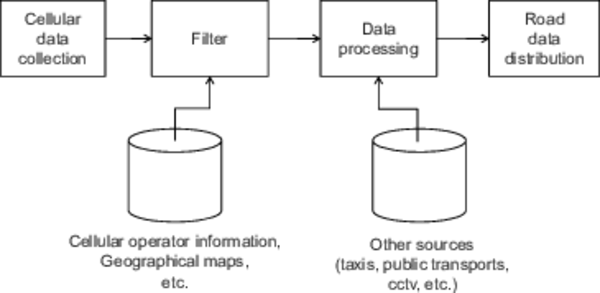
\includegraphics[width=0.7\linewidth]{./images/roadcell}
\caption{RoadCell System Overview \cite{Valerio2009}}
\label{fig:roadcell}
\end{figure}

During their research they found out that a combination of passive and active tracking is best to observe road conditions. Passive tracking is done without the involvement of the mobile station. This approach only utilizes the events captured in the operators core network. While passive tracking offers a high penetration and no increase in network load, it is less accurate than active tracking. Active tracking requires the mobile station and core network to exchange special events that allow the network operator to get an accurate position of the mobile station. This technique is known as Time Difference of Arrival (TDOA). Valerios proposal is to use a combination of both; passive tracking is always used and once the system detects a possible accident active tracking is used for the area in which the accident occurred. This approach improves the accuracy while trying to minimize the additional network load introduced by active tracking.


\subsubsection{Differences and Contribution}
Our approach utilizes handover events. Consecutive Handovers during a call will be combined to a handover sequence. This sequence will be used to model the subscriber mobility. Handovers allow the subscriber to move from the coverage of one cell site to another while still maintaining an ongoing call or data transfer. By estimating the origin of each handover event a trajectory can be computed. The computed trajectory represents the subscriber route. The time of occurrence of a handover event is used as the timestamp. Timestamps in combination with the route will later be used to compute the average velocity for each route segment between two consecutive handover events. Thus, the system can only compute the average velocity for each route segment; the smaller the coverage area of succeeding handovers is, the more accurate the velocity will be. The main limitation of our approach is that it only works for subscriber in connected mode. Therefore, it can only be used to generate trajectories for subscribers during a call. However, this limitation is not a drawback for network simulation since most of the traffic is produced by connected subscribers.
This approach allows mobile network operators to test their mobile networks with simulations based on subscriber behavior. The benefit is that trajectories can be generated for each day of the year. Therefore, this approach can be used to investigate, how changes in the network infrastructure deal with recent scenarios. Annotating the derived route with timing information is an important figure as it influences the network load and traffic. 
